\documentclass[10pt]{beamer}

\usetheme{metropolis}
\usepackage{appendixnumberbeamer}

\usepackage{graphicx}
\usepackage{tikz}
\usetikzlibrary{tikzmark,positioning}
\usepackage{booktabs}
\usepackage[scale=2]{ccicons}

\usepackage{pgfplots}
\usepgfplotslibrary{dateplot}

\usepackage{xspace}
\newcommand{\themename}{\textbf{\textsc{metropolis}}\xspace}

\title{Tomograf\'ia \'optica usando la ecuaci\'on de transferencia radiativa 
independente del tiempo}
\subtitle{... o la dif\'icil tarea de predecir fotones.}
\date{\today}
\author{Alejandra Mendez}
\institute{Instituto de Astronom\'ia y F\'isica del Espacio}
% \titlegraphic{\hfill\includegraphics[height=1.5cm]{logo.pdf}}

\begin{document}

\maketitle

\begin{frame}{Contenido}
  \setbeamertemplate{section in toc}[sections numbered]
  \tableofcontents[hideallsubsections]
\end{frame}
%%%%%%%%%%%%%%%%%%%%%%%%%%%%%%%%%%%%%%%%%%%%%%%%%%%%%%%%%%%%%%%%%%%%%%%%%%
%%%%%%%%%%%%%%%%%%%%%%%%%%%%%%%%%%%%%%%%%%%%%%%%%%%%%%%%%%%%%%%%%%%%%%%%%%
%%%%%%%%%%%%%%%%%%%%%%%%%%%%%%%%%%%%%%%%%%%%%%%%%%%%%%%%%%%%%%%%%%%%%%%%%%
\section{Introducci\'on}
%%%%%%%%%%%%%%%%%%%%%%%%%%%%%%%%%%%%%%%%%%%%%%%%%%%%%%%%%%%%%%%%%%%%%%%%%%
\begin{frame}[fragile]{Tomograf\'ia \'optica (OT)}

\begin{itemize}[<+- | alert@+>]
%  \item \alert<4>{This is\only<4>{ really} important}
 \item Reconstrucci\'on de la distribuci\'on espacial de las propiedades
 \'opticas de materiales dispersivos
 \item Medici\'on de intensidades transmitidas y/o reflejadas en la 
 superficie del material
 \item IR cercano: 650 nm $<\lambda<$ 900 nm
 
\end{itemize}

\end{frame}
%%%%%%%%%%%%%%%%%%%%%%%%%%%%%%%%%%%%%%%%%%%%%%%%%%%%%%%%%%%%%%%%%%%%%%%%%%
\begin{frame}[fragile]{Tomograf\'ia \'optica}



\begin{tikzpicture}
\node[inner sep=0pt] (oceano) at (0,0)
    {\includegraphics[width=0.6\textwidth]{figuras/intro/oceano.jpg}};
    \pause
\node[inner sep=0pt] (ciclon) at (2,1)
    {\includegraphics[width=0.6\textwidth]{figuras/intro/ciclon.jpg}};
    \pause
\node[inner sep=0pt] (ciclon) at (4,2)
    {\includegraphics[width=0.6\textwidth]{figuras/intro/astronomia-inca.png}};
    \pause
\node[inner sep=0pt] (ciclon) at (6,-1)
    {\includegraphics[width=0.4\textwidth]{figuras/intro/neutrones}};
    \pause
\node[inner sep=0pt] (ciclon) at (2,-1.5)
    {\includegraphics[width=0.5\textwidth]{figuras/intro/cerebro.jpg}};
\end{tikzpicture}

\end{frame}
%%%%%%%%%%%%%%%%%%%%%%%%%%%%%%%%%%%%%%%%%%%%%%%%%%%%%%%%%%%%%%%%%%%%%%%%%%
\section{La ecuaci\'on de transferencia radiativa}
%%%%%%%%%%%%%%%%%%%%%%%%%%%%%%%%%%%%%%%%%%%%%%%%%%%%%%%%%%%%%%%%%%%%%%%%%%
\begin{frame}{Transporte de fotones en medios dispersivos}

% \vspace{-3cm}
Ecuaci\'on de transferencia radiativa independiente del tiempo:
\[
\omega\nabla\Psi(\mathbf{r},\omega)+(\tikzmark{mua}\mu_a+\tikzmark{mus}\mu_s)
\tikzmark{psi}\Psi(\mathbf{r},\omega) =S(\mathbf{r},\omega) + 
 \mu_s\int_0^{2\pi}\tikzmark{funp}p(\omega,\omega')\Psi(\mathbf{r},\omega')\,d\omega'\,.
\]


\begin{tikzpicture}[remember picture,overlay,
  expl/.style={draw=orange,fill=orange!30,rounded corners,text width=3.75cm},
  arrow/.style={red!80!black,ultra thick,->,>=latex}
]
\node<2->[expl] 
  (psiex) at (5.5,-0.2cm) {Radiancia [W cm$^{-2}$ sr$^{-1}$]};
\node<3->[expl] 
  (muaex) at (1.2,-1.2cm) {Coeficiente de absorci\'on};
\node<4->[expl] 
  (musex) at (3.5,-2cm) {Coeficiente de dispersi\'on};
\node<5->[expl,text width=4.35cm] 
  (funpex) at (8.5,-1.7cm) {Fase de dispersi\'on: \\
  $p(\cos\theta)=\frac{1-g^2}{2(1+g^2-2g\cos\theta)^{3/2}}$};
\draw<2->[arrow]
  (psiex.north) to[out=135,in=-90] ([xshift=1ex, yshift=-0.5ex]{pic cs:psi});  
\draw<3->[arrow]
  (muaex.north) to[out=90,in=-90] ([xshift=1ex, yshift=-0.5ex]{pic cs:mua});  
\draw<4->[arrow]
  (musex.north) to[out=90,in=-90] ([xshift=1ex, yshift=-0.5ex]{pic cs:mus}); 
\draw<5->[arrow]
  (funpex.north) to[out=90,in=-90] ([xshift=1ex, yshift=-0.5ex]{pic cs:funp});
\end{tikzpicture}

\pause
\vspace{2.5cm}
Se define la fluencia (densidad de energ\'ia):
\begin{equation*}
 \Phi(\mathbf{r})=\int_{2\pi}\Psi(\mathbf{r},\omega)\,d\omega\,.
\end{equation*}

\end{frame}
%%%%%%%%%%%%%%%%%%%%%%%%%%%%%%%%%%%%%%%%%%%%%%%%%%%%%%%%%%%%%%%%%%%%%%%%%%
\section{Set-up experimental}
%%%%%%%%%%%%%%%%%%%%%%%%%%%%%%%%%%%%%%%%%%%%%%%%%%%%%%%%%%%%%%%%%%%%%%%%%%
{%
\setbeamertemplate{frame footer}{Klose et al. 
J Quant Spectrosc Radiat Transf 72 (2002) 691-713}
\begin{frame}[fragile]{Set-up experimental}

\begin{figure}
 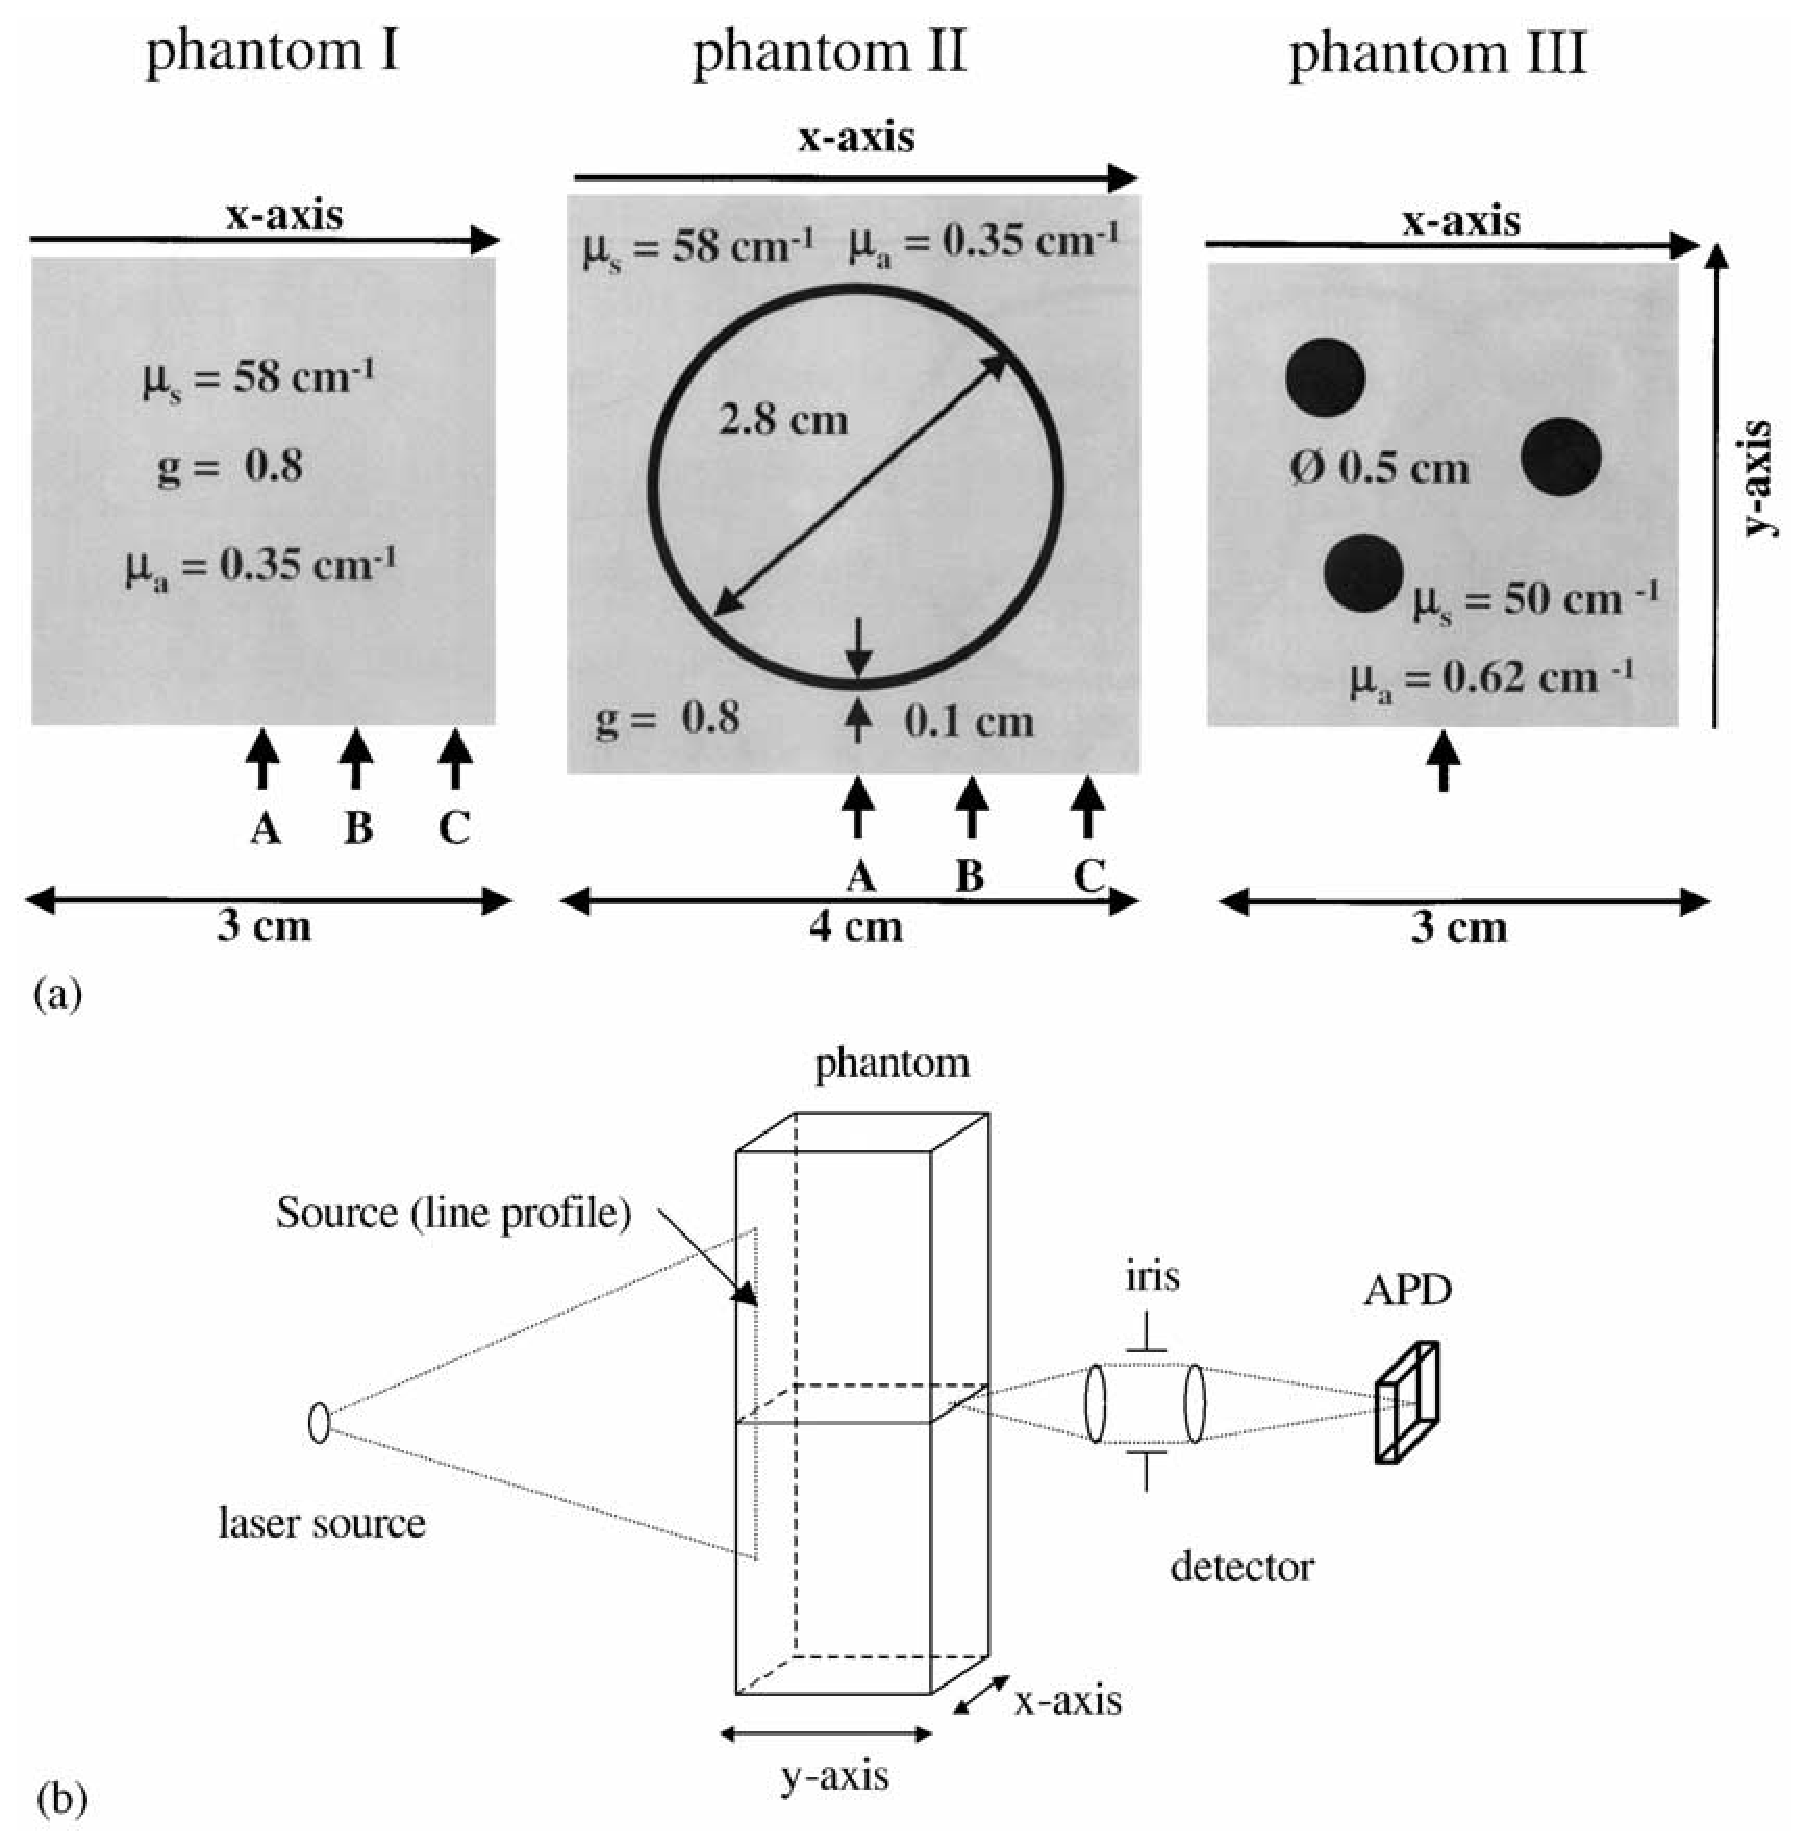
\includegraphics[trim={0 0 0 17cm},clip,width=\textwidth]{fig1.eps}
\end{figure}

\end{frame}
}
%%%%%%%%%%%%%%%%%%%%%%%%%%%%%%%%%%%%%%%%%%%%%%%%%%%%%%%%%%%%%%%%%%%%%%%%%%
\begin{frame}[fragile]{Set-up experimental}

\begin{figure}
 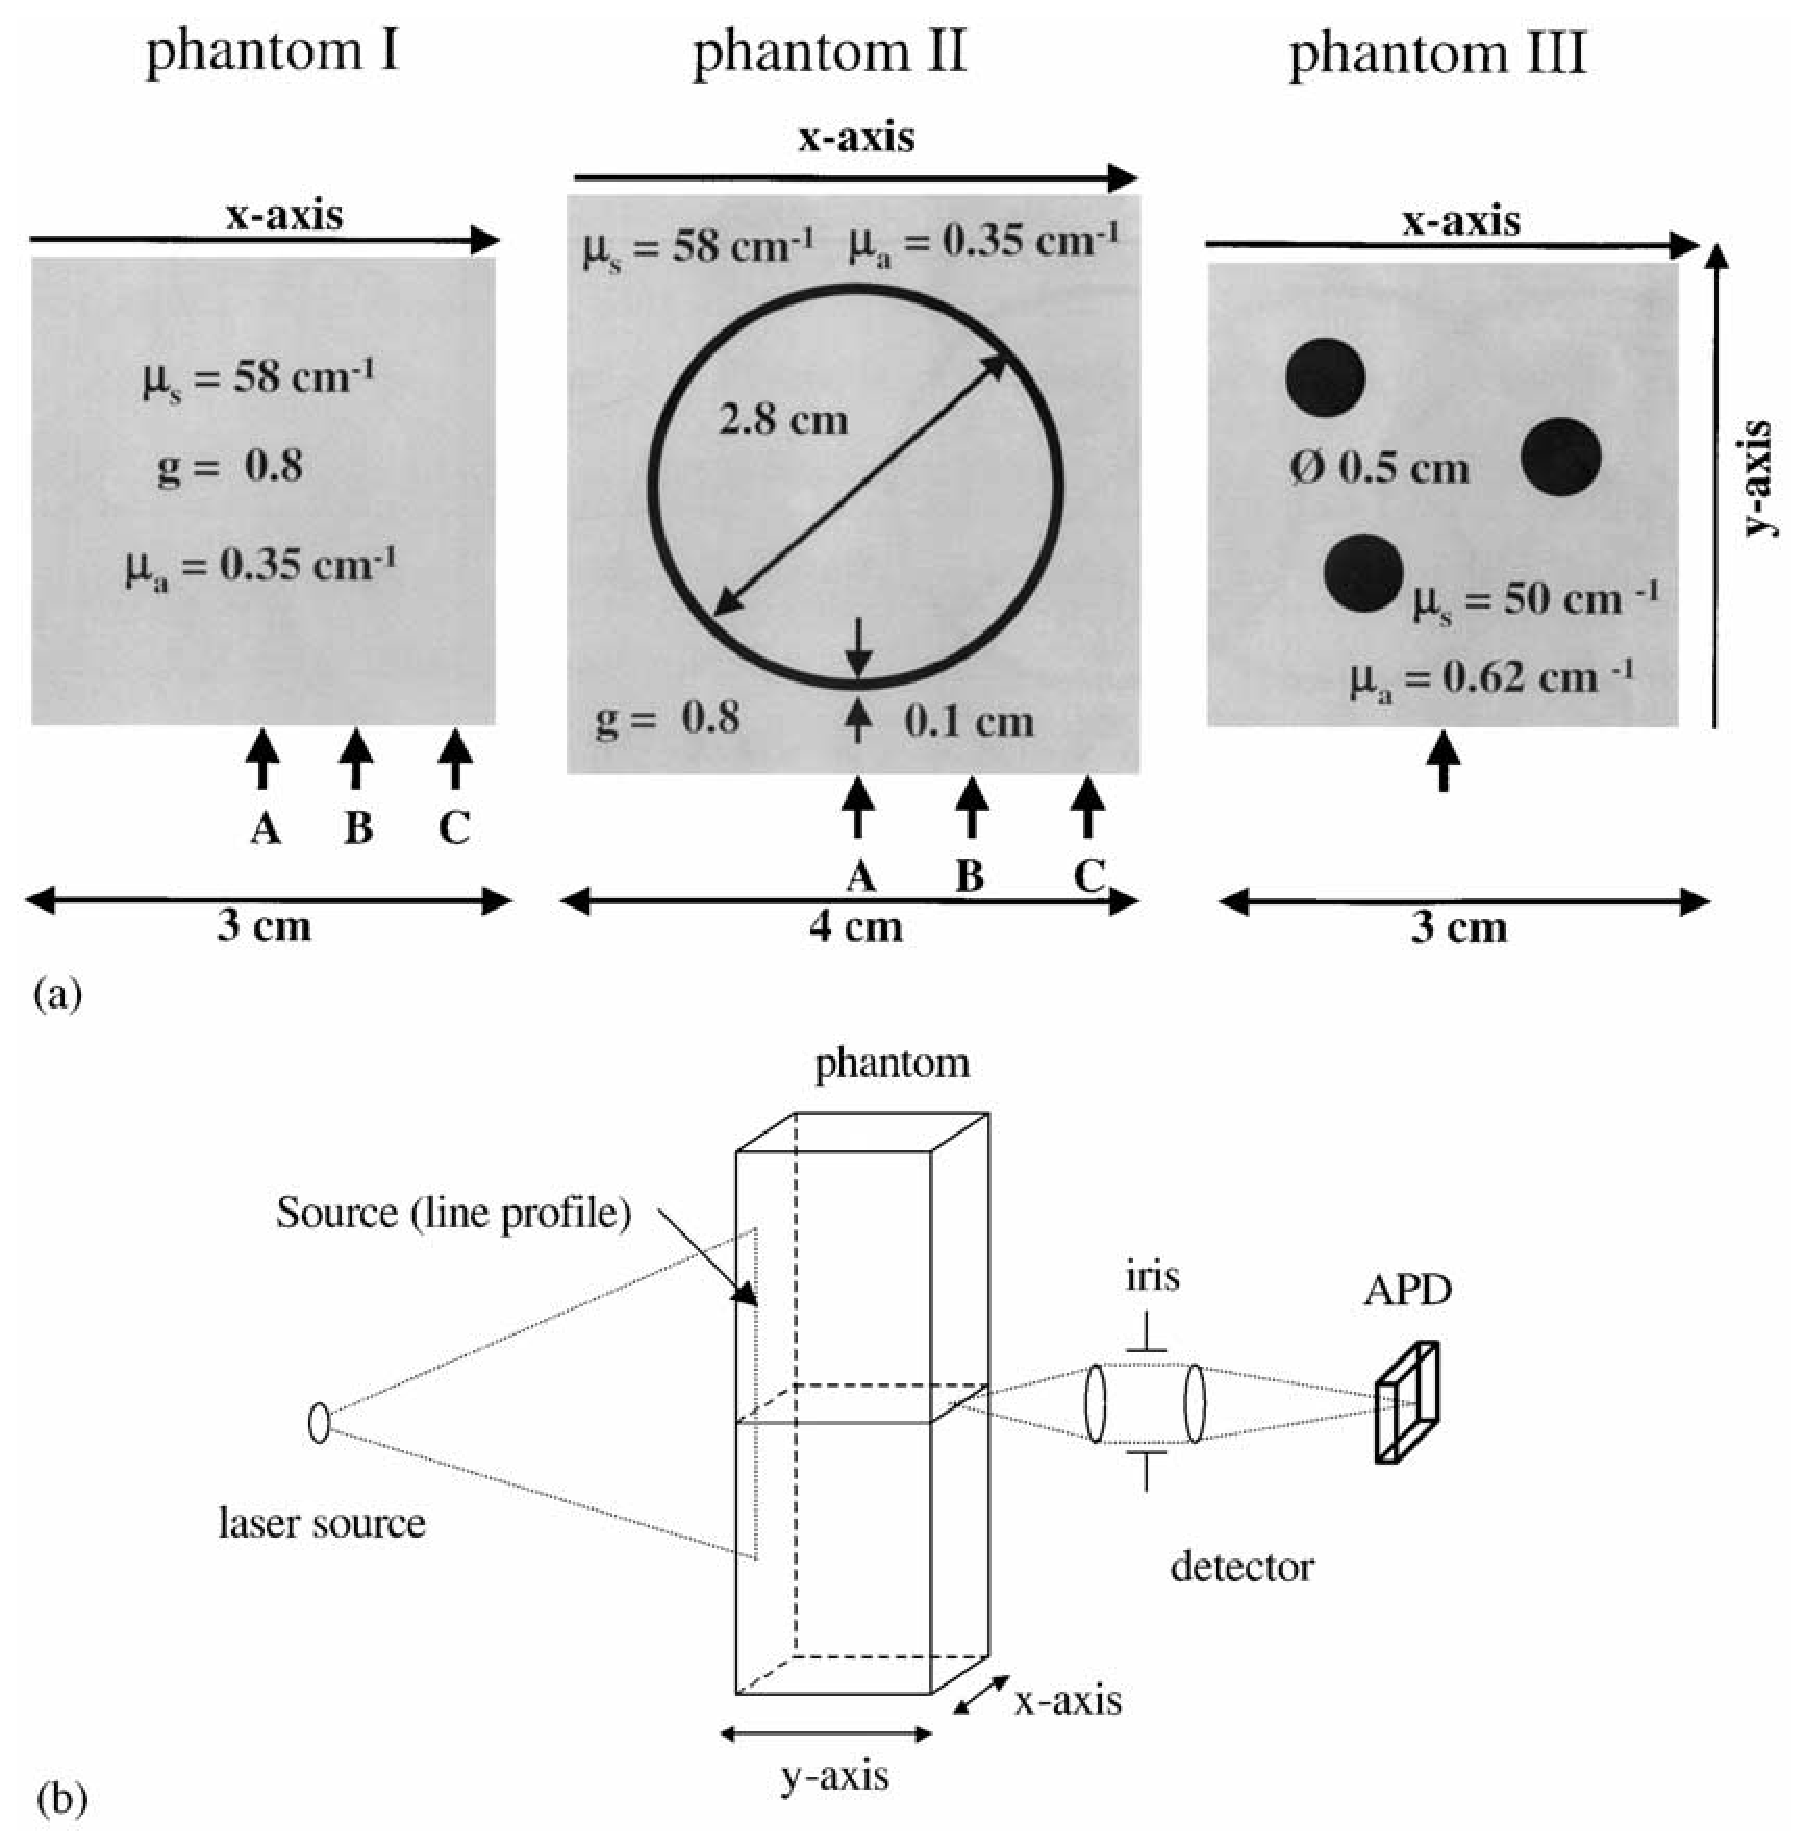
\includegraphics[trim={0 0 0 17cm},clip,width=0.7\textwidth]{fig1.eps}
\end{figure}
\begin{itemize}
 \item Laser diodo de infrarrojo cercano a 678 nm.
 \item Generador de frecuencia provee una modulaci\'on sinusoidal para
 el l\'aser de diodo con 1014 Hz.
 \item Phantom especialmente dise\~nados, con $\mu_s$, $\mu_a$ y $g$ conocidos, homog\'eneos y con estructuras internas.
 \item Fotodiodo de avalancha (APD) 
 \item Amplificador lock-in para mejorar la tasa se\~nal-ruido.
\end{itemize}

\end{frame}
%%%%%%%%%%%%%%%%%%%%%%%%%%%%%%%%%%%%%%%%%%%%%%%%%%%%%%%%%%%%%%%%%%%%%%%%%%
\begin{frame}[fragile]{Fotodiodo de avalancha}

\begin{figure}
 \includegraphics[width=0.5\textwidth]{figuras/Diodo_avalancha.jpg}
\end{figure}
\pause
\begin{equation*}
M=\frac{1}{1-\int_0^L \alpha(x)\,dx}
\end{equation*}

\end{frame}
%%%%%%%%%%%%%%%%%%%%%%%%%%%%%%%%%%%%%%%%%%%%%%%%%%%%%%%%%%%%%%%%%%%%%%%%%%
%\begin{frame}[fragile]{Amplificador lock-in}

%\begin{figure}
% \includegraphics[width=0.5\textwidth]{}
%\end{figure}

%\end{frame}
%%%%%%%%%%%%%%%%%%%%%%%%%%%%%%%%%%%%%%%%%%%%%%%%%%%%%%%%%%%%%%%%%%%%%%%%%%
\begin{frame}[fragile]{Resultados deseados}

\begin{figure}
 \includegraphics[width=0.5\textwidth]{resultado.png}
\end{figure}

\end{frame}
%%%%%%%%%%%%%%%%%%%%%%%%%%%%%%%%%%%%%%%%%%%%%%%%%%%%%%%%%%%%%%%%%%%%%%%%%%
%\section{Resumiendo}

%\begin{frame}{Resumiendo}

%   Get the source of this theme and the demo presentation from
% 
%   \begin{center}\url{github.com/matze/mtheme}\end{center}
% 
%   The theme \emph{itself} is licensed under a
%   \href{http://creativecommons.org/licenses/by-sa/4.0/}{Creative Commons
%   Attribution-ShareAlike 4.0 International License}.
% 
%   \begin{center}\ccbysa\end{center}

%\end{frame}


% \begin{frame}{Font feature test}
%   \begin{itemize}
%     \item Regular
%     \item \textit{Italic}
%     \item \textsc{Small Caps}
%     \item \textbf{Bold}
%     \item \textbf{\textit{Bold Italic}}
%     \item \textbf{\textsc{Bold Small Caps}}
%     \item \texttt{Monospace}
%     \item \texttt{\textit{Monospace Italic}}
%     \item \texttt{\textbf{Monospace Bold}}
%     \item \texttt{\textbf{\textit{Monospace Bold Italic}}}
%   \end{itemize}
% \end{frame}
%%%%%%%%%%%%%%%%%%%%%%%%%%%%%%%%%%%%%%%%%%%%%%%%%%%%%%%%%%%%%%%%%%%%%%%%%%
% \begin{frame}{Lists}
%   \begin{columns}[T,onlytextwidth]
%     \column{0.33\textwidth}
%       Items
%       \begin{itemize}
%         \item Milk \item Eggs \item Potatoes
%       \end{itemize}
% 
%     \column{0.33\textwidth}
%       Enumerations
%       \begin{enumerate}
%         \item First, \item Second and \item Last.
%       \end{enumerate}
% 
%     \column{0.33\textwidth}
%       Descriptions
%       \begin{description}
%         \item[PowerPoint] Meeh. \item[Beamer] Yeeeha.
%       \end{description}
%   \end{columns}
% \end{frame}
%%%%%%%%%%%%%%%%%%%%%%%%%%%%%%%%%%%%%%%%%%%%%%%%%%%%%%%%%%%%%%%%%%%%%%%%%%
% \begin{frame}{Animation}
%   \begin{itemize}[<+- | alert@+>]
%     \item \alert<4>{This is\only<4>{ really} important}
%     \item Now this
%     \item And now this
%   \end{itemize}
% \end{frame}
%%%%%%%%%%%%%%%%%%%%%%%%%%%%%%%%%%%%%%%%%%%%%%%%%%%%%%%%%%%%%%%%%%%%%%%%%%
% \begin{frame}{Figures}
%   \begin{figure}
%     \newcounter{density}
%     \setcounter{density}{20}
%     \begin{tikzpicture}
%       \def\couleur{alerted text.fg}
%       \path[coordinate] (0,0)  coordinate(A)
%                   ++( 90:5cm) coordinate(B)
%                   ++(0:5cm) coordinate(C)
%                   ++(-90:5cm) coordinate(D);
%       \draw[fill=\couleur!\thedensity] (A) -- (B) -- (C) --(D) -- cycle;
%       \foreach \x in {1,...,40}{%
%           \pgfmathsetcounter{density}{\thedensity+20}
%           \setcounter{density}{\thedensity}
%           \path[coordinate] coordinate(X) at (A){};
%           \path[coordinate] (A) -- (B) coordinate[pos=.10](A)
%                               -- (C) coordinate[pos=.10](B)
%                               -- (D) coordinate[pos=.10](C)
%                               -- (X) coordinate[pos=.10](D);
%           \draw[fill=\couleur!\thedensity] (A)--(B)--(C)-- (D) -- cycle;
%       }
%     \end{tikzpicture}
%     \caption{Rotated square from
%     \href{http://www.texample.net/tikz/examples/rotated-polygons/}{texample.net}.}
%   \end{figure}
% \end{frame}
% \begin{frame}{Tables}
%   \begin{table}
%     \caption{Largest cities in the world (source: Wikipedia)}
%     \begin{tabular}{@{} lr @{}}
%       \toprule
%       City & Population\\
%       \midrule
%       Mexico City & 20,116,842\\
%       Shanghai & 19,210,000\\
%       Peking & 15,796,450\\
%       Istanbul & 14,160,467\\
%       \bottomrule
%     \end{tabular}
%   \end{table}
% \end{frame}
% \begin{frame}{Blocks}
%   Three different block environments are pre-defined and may be styled with an
%   optional background color.
% 
%   \begin{columns}[T,onlytextwidth]
%     \column{0.5\textwidth}
%       \begin{block}{Default}
%         Block content.
%       \end{block}
% 
%       \begin{alertblock}{Alert}
%         Block content.
%       \end{alertblock}
% 
%       \begin{exampleblock}{Example}
%         Block content.
%       \end{exampleblock}
% 
%     \column{0.5\textwidth}
% 
%       \metroset{block=fill}
% 
%       \begin{block}{Default}
%         Block content.
%       \end{block}
% 
%       \begin{alertblock}{Alert}
%         Block content.
%       \end{alertblock}
% 
%       \begin{exampleblock}{Example}
%         Block content.
%       \end{exampleblock}
% 
%   \end{columns}
% \end{frame}
% \begin{frame}{Math}
%   \begin{equation*}
%     e = \lim_{n\to \infty} \left(1 + \frac{1}{n}\right)^n
%   \end{equation*}
% \end{frame}
% \begin{frame}{Line plots}
%   \begin{figure}
%     \begin{tikzpicture}
%       \begin{axis}[
%         mlineplot,
%         width=0.9\textwidth,
%         height=6cm,
%       ]
% 
%         \addplot {sin(deg(x))};
%         \addplot+[samples=100] {sin(deg(2*x))};
% 
%       \end{axis}
%     \end{tikzpicture}
%   \end{figure}
% \end{frame}
% \begin{frame}{Bar charts}
%   \begin{figure}
%     \begin{tikzpicture}
%       \begin{axis}[
%         mbarplot,
%         xlabel={Foo},
%         ylabel={Bar},
%         width=0.9\textwidth,
%         height=6cm,
%       ]
% 
%       \addplot plot coordinates {(1, 20) (2, 25) (3, 22.4) (4, 12.4)};
%       \addplot plot coordinates {(1, 18) (2, 24) (3, 23.5) (4, 13.2)};
%       \addplot plot coordinates {(1, 10) (2, 19) (3, 25) (4, 15.2)};
% 
%       \legend{lorem, ipsum, dolor}
% 
%       \end{axis}
%     \end{tikzpicture}
%   \end{figure}
% \end{frame}
% \begin{frame}{Quotes}
%   \begin{quote}
%     Veni, Vidi, Vici
%   \end{quote}
% \end{frame}

% {%
% \setbeamertemplate{frame footer}{My custom footer}
% \begin{frame}[fragile]{Frame footer}
%     \themename defines a custom beamer template to add a text to the footer. It can be set via
%     \begin{verbatim}\setbeamertemplate{frame footer}{My custom footer}\end{verbatim}
% \end{frame}
% }

% \begin{frame}{References}
%   Some references to showcase [allowframebreaks] \cite{knuth92,ConcreteMath,Simpson,Er01,greenwade93}
% \end{frame}

% \section{Resumiendo}

% \begin{frame}{Resumiendo}

%   Get the source of this theme and the demo presentation from
% 
%   \begin{center}\url{github.com/matze/mtheme}\end{center}
% 
%   The theme \emph{itself} is licensed under a
%   \href{http://creativecommons.org/licenses/by-sa/4.0/}{Creative Commons
%   Attribution-ShareAlike 4.0 International License}.
% 
%   \begin{center}\ccbysa\end{center}

% \end{frame}

% \begin{frame}[standout]
%   Questions?
% \end{frame}

% \appendix

% \begin{frame}[fragile]{Backup slides}
%   Sometimes, it is useful to add slides at the end of your presentation to
%   refer to during audience questions.
% 
%   The best way to do this is to include the \verb|appendixnumberbeamer|
%   package in your preamble and call \verb|\appendix| before your backup slides.
% 
%   \themename will automatically turn off slide numbering and progress bars for
%   slides in the appendix.
% \end{frame}

% \begin{frame}[allowframebreaks]{References}
% 
%   \bibliography{demo}
%   \bibliographystyle{abbrv}
% 
% \end{frame}

\end{document}
